% ==========================================================
\section{Integrating Behavioral Programming into UVL}
\label{sec:concept_bp_integration}
% ==========================================================

This section describes, at a conceptual level, how Behavioral Programming can be integrated into the \gls{uvl}-based language and its available tooling.
The objective is to extend the language and tools so that models can express \gls{bp} event constraints and \gls{bp}-specific top-level features while preserving \gls{uvl}'s core philosophy and backward compatibility.

% ----------------------------------------------------------
\subsection{ANTLR grammar extensions: \texttt{uvl-parser}}
\label{subsec:concept_bp_integration_antlr}
% ----------------------------------------------------------

As described in Section~\ref{subsec:fmbp}, FMBP already implements an extension of \gls{uvls} to represent \gls{bp}-specific semantics.
\gls{uvls} is based on the tree-sitter parsing library~\cite{loth_uvls_2023}, which did not require any grammar modifications to support the \gls{bp} constructs~\cite{felber_comprehensible_2025, felber_tfelbruvl-bp-lsp_2025}.
For this work, the \texttt{uvl-parser} is used instead~\cite{sundermann_uvlparser_2023, noauthor_universal-variability-languageuvl-parser_2026}, which is based on \gls{antlr}~\cite{noauthor_antlrantlr4_2026}.
The \texttt{uvl-parser} library is also used in the \gls{uvl} integration of FeatureIDE~\cite{noauthor_featureidefeatureide_2026}.
\gls{antlr} is a parser generator that takes a formal grammar as input and produces a parser in a target host language~\cite{parr_definitive_2013}.
The \texttt{uvl-parser} provides the \gls{antlr} grammar files that define \gls{uvl}'s concrete syntax and supports Java as a target language besides Python and JavaScript~\cite{noauthor_universal-variability-languageuvl-parser_2026}.
Although both the tree-sitter-based and \gls{antlr}-based parsers represent the same language, their definitions of the concrete syntax differ.
The \gls{bp} constructs introduced by Felber and Götz~\cite{felber_behavioral_2025} are not currently supported by the \texttt{uvl-parser}, so the grammar must be extended to accommodate them.

According to the \gls{antlr} grammar file, \gls{uvl} permits a single top-level feature at the model root~\cite{noauthor_universal-variability-languageuvl-parser_2026}.
An example of such a grammar rule is shown in Listing~\ref{lst:antlr-top-level-feature}.
\gls{bp} models extend this by requiring two additional, named top-level features at the root: \texttt{Env} and \texttt{Config}.
Due to the grammar definition, it currently rejects models that place \texttt{Env} or \texttt{Config} next to the common feature model root, for example, the \gls{uvl} model shown in Listing~\ref{lst:drone_uvl}.
To support \gls{bp} while preserving compatibility, the grammar must be extended so these two required top-level features are accepted in a backward-compatible way.
Importantly, this allowance must be limited to the default single top-level feature plus the two \gls{bp}-specific sections, and must not permit arbitrary additional top-level features.
Standard \gls{uvl} models that do not include these features should continue to parse unchanged when \gls{bp} parsing is not enabled.

\lstinputlisting[
    float,
    floatplacement=ht,
    caption={Excerpt from the \texttt{uvl-parser} grammar showing the restriction for a single top-level feature.},
    label={lst:antlr-top-level-feature}
]{code/concept/uvl_grammar_snippet.g4}

The existing constraints defined in the \texttt{uvl-parser} grammar are shaped around classical \gls{uvl} constraint forms.
They include Boolean and mathematical combinations, common expressions and functions (e.g., sum aggregates), and cross-tree relations between features~\cite{noauthor_universal-variability-languageuvl-parser_2026}.
The base grammar already includes single-reference constraint shapes for these use cases so that this approach can be reused for \gls{bp}-specific single-reference constraints such as \texttt{requested}, \texttt{waited\_for}, \texttt{blocked}, and \texttt{selected}.
Reusing that approach may require lexical disambiguation for the event-role names so they can appear unambiguously as attribute identifiers.
In contrast, \texttt{conflicting} is a true multi-reference constraint that binds several feature references simultaneously and is not covered by existing single-reference forms.
To support it, an explicit multi-reference production must be added to the grammar.
These \gls{bp}-specific constraints should be grouped as a distinct alternative, accepted only when \gls{bp} parsing is enabled, so they do not interfere with the existing constraint forms.
B-threads and b-events themselves are already representable in the grammar as attributes of features and do not require changes to the existing rules.
Their semantics can be handled by the \gls{glsp} server or other tooling after successful parsing.
Taken together, these grammar changes provide the syntactic basis needed to extend the language in a way that advances RQ2.

% ----------------------------------------------------------
\subsection{Java metamodel extensions: \texttt{java-fm-metamodel}}
\label{subsec:concept_bp_integration_metamodel}
% ----------------------------------------------------------

The \texttt{java-fm-featuremodel} hosts the Java source model classes and the parser-to-model factories that translate \gls{antlr} parse trees into typed feature model objects~\cite{noauthor_universal-variability-languagejava-fm-metamodel_2026}.
Due to its coupling with the \texttt{uvl-parser}, it must be extended to support the new grammar constructs introduced for \gls{bp}.

The metamodel must distinguish between an existing class, \texttt{FeatureModel}, and a \gls{bp}-specific class, \texttt{BPFeatureModel}.
It allows the \gls{glsp} server to be deployed as two distinct variants, one targeting plain \gls{uvl} authoring and one targeting \gls{bp}-enhanced authoring, each activating only the capabilities relevant to its context.
Therefore, we create the \texttt{BPFeatureModel}, which subclasses the base \texttt{FeatureModel}.
The class must include additional fields for the \texttt{Env} and \texttt{Config} top-level features, enabling direct access to these contextual elements.
Consumers that work exclusively with the base class remain entirely unaware of the \gls{bp} extension and require no modification.
Figure~\ref{fig:bp-class-diagram} displays a concept of the extended setup.

\begin{figure}
	\centering
	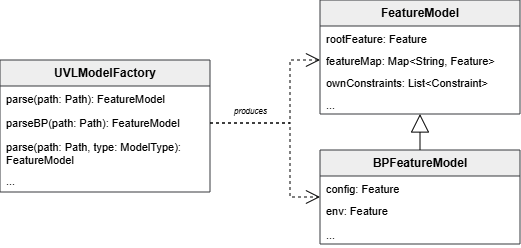
\includegraphics[width=0.9\textwidth]{figures/uml_feature-model.png}
	\caption{Simplified class diagram showing \texttt{FeatureModel} as the base class and \texttt{BPFeatureModel} as its extension; both classes are produced by \texttt{UVLModelFactory}.}
    \label{fig:bp-class-diagram}
\end{figure}

\gls{bp} introduces constraint semantics that cannot be represented by the existing constraint classes~\cite{noauthor_universal-variability-languagejava-fm-metamodel_2026}.
An abstract base class can be added to the metamodel to represent the general concept of a \gls{bp}-specific constraint, with concrete subclasses for each specific constraint type.
Additionally, the \texttt{Conflicting} subclass should support multiple references.

The model factory and parser listener must be extended to instantiate these objects when \gls{bp} parse nodes are encountered. 
For example, the listener must recognize the new top-level feature rules and attach them to the \texttt{BPFeatureModel} when \gls{bp} parsing is enabled.
The existing unit tests for the \texttt{java-fm-metamodel} should be extended to cover the new \gls{bp} constructs.

The extended metamodel supports both parsing of default \gls{uvl} models and parsing of new \gls{bp}-enhanced models, thereby answering RQ2 of this thesis.